
\documentclass[a4paper,12pt]{report}


\usepackage[english,romanian]{babel}
\usepackage{pgfpages}
\usepackage{graphicx}

\usepackage{ucs}
\usepackage[utf8x]{inputenc}
% 
% \newcommand{\texten}[1]{\foreignlanguage{english}{#1}}
% \newcommand{\textro}[1]{\foreignlanguage{romanian}{#1}}
% 
% \newcommand{\sh}[0]{\textcommabelow{s}}		%pentru ş cu virgulă
% \newcommand{\tz}[0]{\textcommabelow{t}}		% pentru ţ cu virgulă

\usepackage[unicode]{hyperref}
\usepackage[T1]{fontenc}
\usepackage{tikz}
% \usepackage{colortbl}
\usepackage{yfonts}

\usepackage{amssymb,amsmath}
\usepackage{amsthm}

\usepackage{paralist}

\usepackage{enumerate}

% \usepackage{makeidx}
% \usepackage{showidx}

\usepackage{multirow}

% \usepackage{float}

% \usepackage{subfig}

% \usepackage{multirow}
% \usepackage{rotating}

% \usepackage[ruled,vlined,longend]{algorithm2e}
% \SetAlFnt{\small}

% \usepackage{program}
\usepackage{algpseudocode}

\usepackage{verbatim}

\usepackage{listings}

\lstset{
	language=C,
%	basicstyle=\ttfamily,
	basicstyle=\small\ttfamily,
	keywordstyle=\bfseries,
	commentstyle=\itshape,
	escapechar=\,
	emphstyle=\bfseries\color{red}
 	commentstyle=\slshape\color{green!50!black},
 	keywordstyle=\bfseries\color{blue!50!black},
 	identifierstyle=\color{blue},
 	stringstyle=\color{orange},
	showstringspaces=false
}

\usepackage{setspace}
% \usepackage{tocbibind}
% \usepackage{fancyhdr}


% \newcommand{\OSName}{\textit{Nachos}}
\newcommand{\OSName}{\textit{HAL9000}}

\title{The Design of \OSName{} Operating System. Light Project}

\author{Students' Name}

% \onehalfspacing

\begin{document}

\selectlanguage{english}
% \selectlanguage{romanian}


\maketitle

\begin{abstract}
The abstract should contain a very short description of the results presented in this report. 

Take into account that a design document is a high-level, logical (abstract) description of the solution you propose to the problems and requirements you dealt with. Though, it should be detailed enough such that somebody who already knows and understands the requirements could implement (i.e. write the code) the design without having to take any significant additional design decisions. Even further, if such an implementer would happen to be an experienced one, he or she should be able to use the design document to implement the solution in just few hours (not necessarily including the debugging). 

\textbf{Important notes}. Take care to remove from the given design document template all the text that was given to you as a guideline and provide your own document with only your own original text. Also, do not simply write anything in any section just to have some text there, but only write text that makes sense in the given context. We will not count the number of pages or words of your document, but will only evaluate the meaning and completeness of the written words. 
\end{abstract}


% \chapter{General Presentation}


% \section{System}


\chapter{The (One) Way to Proceed for Getting a Reasonable Design}

\section{General Considerations}

There are multiple strategies to develop a software application, though basically all of them comprise the following four phases:
\begin{enumerate}
    \item establish the \textit{application requirements} or specification;
    \item derive the ways the requirements can be realized / satisfied, i.e. \textit{designing} the application;
    \item \textit{implement} the design, e.g. write the corresponding code;
    \item check if the implementation satisfies the specification, at least by \textit{testing} (as exhaustive as possible) the developed application.
\end{enumerate}

In practice, a perfect and complete design is not entirely possible from the beginning for most of the projects. So, at least the last three phases actually correspond to a progressive and repeating process, i.e. make a first design, implement it, test the resulting code, see what is working bad or missing functionality, go back and change the design, make the corresponding code changes or additions, test them again and so on. 

I want, however, to warn you that even if we cannot make a perfect design from the beginning that does not mean that we do not have to make any design at all and just start writing code. This is a really bad idea. And actually, in my opinion, when you start writing code without a more or less formal design, what you actually have to do is to derive an on-the-fly design. What I mean is that you cannot just write ``some'' code there, hoping to get the required functionality. You must think of \textit{how} to code and \textit{what} code to write and this is basically a (hopefully, logical) plan, i.e. a design. Such a strategy, however, results most of the time and for most of the people in just poorly improvisation and requires many returns to the ``design'' phase to change data structures and code. In short, a lot of lost time and bad results. 

Coming back to the idea that we cannot make a complete design from the beginning, there are a few ways to understand this and reasons of having it. Firstly, it is generally difficult to cover all the particular cases, especially for very complex systems and requirements. That means that what you get first is a sort of a general design, establishing the main components of your application and their basic interrelationships. It is not surely that you immediately could start writing code for such a design, but it is very possible to be able to write some prototype, just to see if your ideas and design components could be linked together. On way or another, the next major step is to go deeper for a more detailed design. Secondly, one reason of not getting a complete design from the beginning is just because you want to concentrate on a particular component firstly, and only than to cope with the others. However, this is just a particular case of the first strategy, because it is not possible to deal with one application component without knowing firstly which are the others and how they depend on one another. Thirdly, maybe it is not needed to get a complete detailed design from the beginning, just because the application components are dealt with by different teams or, like in your case, different team members. It is not needed in such a case to deal with the complexity of each application component from the beginning, as each one be will be addressed latter by its allocated team (members), but just try to establish as precise as possible, which are the application components and how they need to interact each other. In your \OSName{} project the application components are most of the time already established, so what remains for you is only to clarify the interactions and interfaces between them. After such a general design, each team (member) can get independently into a more detailed design of his/her allocated application component. 
In conclusion, you need to derive at least a general design before starting writing any code and refine that design later. 

Take into  account, however, that in or project we have distinct deadlines for both design and implementation phases, and that you will be graded for the two relatively independent (thus, design regrading will be done only occasionally). This means that you have to try to derive a very good and as detailed as possible design from the beginning.  


Another practical idea regarding the application development phases is that there is no clear separation between those phases and especially between the design and implementation ones. This means that during what we call the design phase we have to decide on some implementation aspects and, similarly, when we are writing code we still have to take some decisions when more implementation alternatives exists (which could influence some of the application non-functional characteristics, like performance) or some unanticipated problems arise. Even taking into account such realities, in this design document we are mainly interested (and so you have to focus) mainly on the design aspects. But, as I said above, I will not expect you providing a perfect design, which would need no changes during its implementation. However, this does not mean that you are free to come with an unrealistic, incoherent, illogical, hasty, superficial design, which does not deal with all the (clear and obvious) given requirements. 

One important thing to keep in mind when you make your design and write your design document is that another team member has to be able to figure out easily what you meant in your design document and implement your design without being forced to take any additional design decisions during its implementation or asking you for clarifications. It is at least your teacher you have to think of when writing your design document, because s/he has to understand what you meant when s/he will be reading your document. Take care that you will be graded for your design document with approximately the same weight as for your implementation. 

Beside the fact that we do not require you a perfect design, and correspondingly we do not grade with the maximum value only perfect designs (yet, please, take care and see again above what I mean by an imperfect design), your design document must also not be a formal document. At the minimum it should be clear and logical and complies the given structure, but otherwise you are free to write it any way you feel comfortable. For example, if you think it helps someone better understand what you mean or helps you better explain your ideas, you are free to make informal hand-made figures, schemes, diagrams, make a photo of them or scan them and insert them in your document. Also, when you want to describe an algorithm or a functionality, you are free to describe it any way it is simpler for you, like for instance as a pseudo-code, or as a numbered list of steps. However, what I generally consider a bad idea is to describe an algorithm as an unstructured text. On one hand, this is difficult to follow and, on the other hand, text could generally be given different interpretations, though as I already mentioned your design should be clear and give no way for wrong interpretation, otherwise it is a bad design. 

Regarding the fact that design and implementation could not be clearly and completely separated, this is even more complicated in your \OSName{} project that you start from a given code of an already functional system. In other words you start with an already partially designed system, which you cannot ignore. This means, on one hand, that you could be restricted in many ways by the existing design and \OSName{} structure and, on the other hand, that you cannot make your design ignoring the \OSName{}' code. Even if, theoretically, a design could be abstract enough to support different implementations (consequently, containing no particular code), your \OSName{} design has to make direct references to some existing data structures and functions, when they are needed for the functionality of the \OSName{} component your are designing. So, do not let your design be too vague (abstract) in regarding to the functionality directly relying on exiting data structures and functions and let it mention them explicitly. For instance, when you need to keep some information about a thread, you can mention that such information will be stored as additional fields of the ``\textit{THREAD}'' data structure. Or, when you need to keep a list of some elements, you have to use the lists already provided by \OSName{} and show that by declaring and defining your list in the way \OSName{} does, like below:

\begin{lstlisting}
	// this is the way HAL9000 declares a generic list
	LIST_ENTRY myCoolList;

	typedef struct _MY_LIST_ELEM {
		... some fields ...

		// this is needed for linking MY_LIST_ELEM in the 
		// myCoolList list
		LIST_ENTRY ListElem;
	} MY_LIST_ELEM, *PMY_LIST_ELEM;
\end{lstlisting}

The next sections illustrate the design document structure we require and describe what each section should refer to.


\section{Application Requirements. Project Specification}

% Describe briefly what you have been given (have started from) at the beginning of the assignment and the way the existing functionality must be extended.

\subsection{``What you have'' and  ``What you have to do''}

In this section you have to make clear what you are required to do for each particular assignment of the \OSName{} project. In the \OSName{} project, you are already given the assignment requirements, so it is not your job to establish them. You must, however, be sure that you clearly understand them. Having no clear idea about what you have to do, gives you a little chance to really get it working. Please, do not hesitate to ask as many questions about such aspects on the \OSName{} forum (on the moodle page of the course) as you need to make all the requirements clear to you. Take care, however, that you have to do this (long enough) before the design deadline, such that to get an answer in time. We will do our best in answering your questions as fast as possible, though we cannot assure you for a certain (maximum) reaction time. You will not excused at all if you say you had not understood some requirements when you will be presenting your design document.

So, for this small section, take a moment and think of and briefly write about: 
\begin{enumerate}
    \item what you are starting from, i.e. what you are given in terms of \OSName{} existing functionality, and
    \item what you are required to do.
\end{enumerate}


\subsection{``How it would be used''}

Making clear the requirements could be helped by figuring some ways the required functionality would be used once implemented. 
For this you have to describe briefly a few common use-cases, which could later be used as some of the implementation tests. 

You could use for this the tests provided with the \OSName{} code in the ``tests/'' subdirectory. Take at least a short look at each test case to identify common cases.


\section{Derive the Application's Design}

Generally, you have to follow a top-down design approach, starting with a particular requirement and identifying the inputs it generates to your application (i.e. \OSName{} OS). Such that you could establish the ``entry (starting) points'' in your system to start your design from. 

Next, you also have to identify the logical objects (i.e. data structures, local and global variables etc.) implied and affected by the analyzed requirement and the operations needed to be performed on them. Also establish if you need to introduce and use additional information (i.e. fields, variables) in order to make such operations possible. 

Once you established the information you need to keep in order to dealt with the analyzed requirement, you could decide on the way to keep track of and manage that data. 
In other words, this is the way you can \textit{identify the needed data structures} and \textit{operations on them}. There could not necessarily be just one solution. For example, at one moment you could use a linked list or a hash table. In order to decide for one or another, you have to figure out which one helps you more, which one fits better for the most frequent operation and other things like these. Once you decided on the data structures, you have to establish where and how they are
\begin{inparaenum}[(1)]
    \item \textit{initialized}, 
    \item \textit{used}, 
    \item \textit{changed}, and finally 
    \item \textit{removed}.
\end{inparaenum}

This way you could identify the places (e.g. other system components, functions) where you have to add the needed functionality. In terms of \OSName{} code you could identify the functions needed to be used, changed or even added. 

As a result of your requirement analysis you could organize your resulting design like below. 

\subsection{Needed Data Structures and Functions}

Describe the \textit{data structures} and \textit{functions} (only their signature and overall functionality) needed by your design and what they are used for. Describe in few words the purpose of new added data structures, fields and functions. As mentioned before, cannot ignore the fact that \OSName{} is written in C. Thus, describe you data structures in the C syntax referring, when the case, to existing data structures, like in the example given above. If you only need to add new fields in existing data structures, mention only the added fields, not all of them. 

\begin{lstlisting}
    typedef struct _EXISTENT_DATA_STRUCTURE {
        ...
        int NewField;
        char NewField2;
        ...
    } EXISTENT_DATA_STRUCTURE, *PEXISTENT_DATA_STRUCTURE;
    
    typedef struct _NEW_DATA_STRUCTURE {
        ... new fields ...
    } NEW_DATA_STRUCTURE, *PNEW_DATA_STRUCTURE;
    
    STATUS NewFunction(void);
\end{lstlisting}


\subsection{Detailed Functionality}

This should be \textbf{the largest and most important section} of you design document. It must describe \textbf{explicitly}, in words and pseudo-code the way your solution works. DO NOT INCLUDE CODE HERE. This is a design document, not a code description one. As much as possible try to describe the design principles, not implementation details. 

Give examples, if you think they can make your explanation clearer. You are free to use any other techniques (e.g. use-case diagrams, sequence diagrams etc.) that you think can make your explanation clearer. See Figure~\ref{fig:sample-image} below to see the way images are inserted in a Latex file. 

\begin{figure}[h]
	\centering
	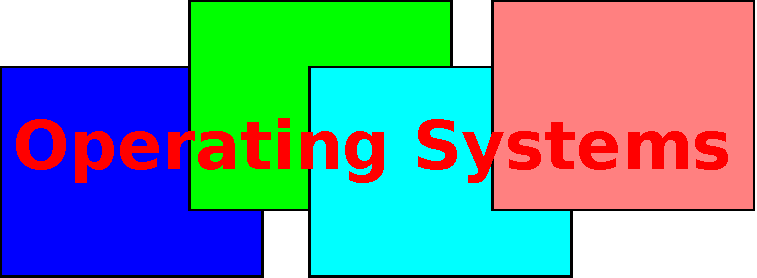
\includegraphics[width=0.5\textwidth]{figures/sample-image.pdf}
	\caption{Sample image}
	\label{fig:sample-image}
\end{figure}

When describing algorithms you are to use or develop, it is very important to also describe them in a formal way, not just as free text description. Commonly, this could be done as a sort of pseudo-code or just as a simple list of logically ordered steps (enumerated list). In your algorithm description you should (i.e. must) refer to the data structures and variables you described in the previous section, following the recommendations in Section~\ref{sec:derive-design}. This way you avoid describing your algorithms too vague and reduce the risks of being misunderstood.  

Here you have a pseudo-code description of an algorithm taken from \\ \href{http://en.wikibooks.org/wiki/LaTeX/Algorithms\_and\_Pseudocode\#Typesetting\_using\_the\_program\_package}{http://en.wikibooks.org/wiki/LaTeX}. It uses the \textit{algpseudocode} package. Alternatively, you can use any other package and environment of same sort you like. 

% \begin{program}
% \mbox{Example of a pseudo-code algorithm description:}
% \BEGIN
%   \FOR i:=1 \TO 10 \STEP 1 \DO
%      |expt|(2,i); \\ |newline|() \OD
% \rcomment{This text will be set flush to the right margin}
% \WHERE
% \PROC |expt|(x,n) \BODY
%           z:=1;
%           \DO \IF n=0 \THEN \EXIT \FI;
%              \DO \IF |odd|(n) \THEN \EXIT \FI;
% \COMMENT{This is a comment statement};
%                 n:=n/2; x:=x*x \OD;
%              \{ n>0 \};
%              n:=n-1; z:=z*x \OD;
%           |print|(z) \ENDPROC
% \END
% \end{program}

\begin{algorithmic}
\If {$i\geq maxval$}
    \State $i\gets 0$
\Else
    \If {$i+k\leq maxval$}
        \State $i\gets i+k$
    \EndIf
\EndIf
\end{algorithmic}

\subsection{Explanation of Your Design Decisions}

Justify very briefly your design decisions, specifying other possible design alternatives, their advantages and disadvantages and mention the reasons of your choice. For instance, you can say that you decided for a simpler and easier to implement alternative, just because you had no enough time to invest in a more complex one. Or just because you felt it would be enough for what \OSName{} tests would check for. This could be viewed as a pragmatical approach and it is not necessarily a bad one, on the contrary, could be very effective in practice.  


\section{Testing Your Implementation}

Please note that the \OSName{} code is provided with a set of tests that are used to check and evaluate your implementation. The \OSName{} tests could be found in the ``tests/'' subdirectory, organized in different subdirectories for each different assignments (like, ``threads'', ``userprog'' etc.).

To find out the names of all the tests to be run for a module you can build the \textit{RunTests} project and wait for execution to finish.

Actually, this is the first command that will be executed on your implementation when graded, so please, do not hesitate do run it by yourself as many times as needed during your \OSName{} development, starting from the design phase. 

In this section you have to describe briefly each of the given \OSName{} tests that will be run in order to check the completeness and correctness of your implementation. 
Take care that your grade is directly dependent on how many tests your implementation will pass, so take time to see if your design take into account all particular usage scenarios generated by all \OSName{} tests. 


\section{Observations}

You can use this section to mention other things not mentioned in the other sections. 

You can (realistically and objectively) indicate and evaluate, for instance:
\begin{itemize}
	\item the most difficult parts of your assignment and the reasons you think they were so; 
	
	\item the difficulty level of the assignment and if the allocated time was enough or not; 

	\item particular actions or hints you think we should do for or give to students to help them better dealing with the assignments.

\end{itemize}

You can also take a minute to think what your achieved experience is after finishing your design and try to share that experience with the others. 

You can also make suggestions for your teacher, relative to the way s/he can assist more effectively her/his students.

If you have nothing to say here, please remove it.



\chapter{Design of Module \textit{Threads}}

\begin{abstract}
    This document contains the design for the changes required to implement the light project specification  of the threads module of the HAL9000 operating system. 
    
    The document was created as a task for the Operating Systems Design subject taught at the Technical University of Cluj-Napoca. 
    
    \textcolor{red}{The document has some sections that are intentionally left for you to fill in. This sections are marked with red. Fill them in before you deliver your assignment.}
    
\end{abstract}


% ================================================================================= %
\section{Assignment Requirement}


% -------------------------------------------------- %
\subsection{Initial Functionality}

    The HAL9000 operating system supports multi-core processors. After boot, each core is allowed to run operating system threads. 
        
    Functions to manage threads are implemented in the \textit{thread.c} file. The \textit{thread.h} file contains a documented public interface for the thread functionality.

    Information about threads are stored internally in the \lstinline|_THREAD| structure defined in \textit{thread\_internal.h}. This structure is reference counted. The \lstinline|_ThreadDestroy| function frees the memory for a \lstinline|_THREAD| structure whenever the reference count of it reaches 0.

    All threads in the system are stored in the \lstinline|m_threadSystemData.AllThreadsList| list. This list is protected by the \lstinline|m_threadSystemData.AllThreadsLock|.

\subsubsection{Thread identifiers}
    A thread'a identifier is stored in the \lstinline|_THREAD| structure as the \lstinline|TID Id| field. 
    
    Code that initializes the Id of each thread is contained inside the \lstinline|_ThreadInit| function:
    \begin{lstlisting}
     pThread->Id = _ThreadSystemGetNextTid();
    \end{lstlisting}
    
    The \lstinline|_ThreadSystemGetNextTid| function is responsible with generating new thread identifiers. Thread identifiers are generated by atomically adding \lstinline{TID_INCREMENT} to the last id generating by the function. The initial implementation sets \lstinline|TID_INCREMENT| to 4. 
    
    Information about the current CPU is stored in the \lstinline|_PCPU| structure defined in \lstinline|cpumu.h| header file. A pointer to the structure corresponding to the current CPU may be obtained using the \lstinline|GetCurrentPcpu| macro. 

\subsubsection{Account for number of threads created}
    The \lstinline|ThreadCreateEx| is used to create new threads to run on HAL900. This function allocates and sets up the \lstinline|_THREAD| structure for the newly created thread. The function is always executed in the context of the parent that creates the thread. 

    The \lstinline|ThreadExit| function is called whenever a thread terminates. HAL9000 assures that this function is always called by wrapping threads inside the \lstinline|_ThreadKernelFunction| function. 
    
\subsubsection{Round robin scheduler}
    HAL9000 implements a round robin scheduler strategy based on timer interrupts. When a timer interrupt is generated on the processor, the interrupt handler eventually calls the \lstinline|ThreadTick| function. If a thread spent more then \lstinline|THREAD_TIME_SLICE| ticks on the processor, the scheduler forces it to yield execution. 
    
    The \lstinline{_ThreadSchedule} function is responsible with selecting the next thread to run on the CPU. 



% -------------------------------------------------- %
\subsection{Requirements}

\subsubsection{Thread identifiers}
We are required to perform two changes:
\begin{itemize}
    \item change the way thread identifiers are allocated, such that the values used for the field Id in structure THREAD to be multiples of 5
    \item store the identifier of the CPU the thread was created on.
\end{itemize}

\subsubsection{Account for number of threads created}

We are required to print two messages as follows. 

On thread creation:  "Thread [ID=NEW\_TH\_ID] is the Xth thread created by thread [ID=CRT\_TH\_ID] on CPU [ID=CRT\_CPU\_ID]", where \lstinline|NEW_TH_ID| is the identifier of the newly created thread, \lstinline|CRT_TH_ID| is the identifier of the currently running thread, and \lstinline|CRT_CPU_ID| is the identifier of the current CPU. 

On thread exit: "Thread [ID=CRT\_TH\_ID] created on CPU [ID=CPU\_ID] is finishing on CPU [ID=CRT\_CPU\_ID], while its parent thread [ID=PR\_TH\_ID] still has more X child threads", where \lstinline|CRT_TH_ID| is the identifier of the currently terminating thread, \lstinline|PR_TH_ID| is the identifier current thread's parent, \lstinline|CPU_ID| is the ID of the CPU the thread was created on, and \lstinline|CRT_CPU_ID| is the ID of the CPU the thread is running during its termination.

For this we need to
\begin{itemize}
    \item know the parent of each thread
    \item count the number of threads created by each parent thread
    \item count the number of still running children of each thread
\end{itemize}


\subsubsection{ Round robin scheduler}

For this task we have three requirements:
\begin{itemize}
    \item allocate a the time quantum of 3 ticks for threads having an odd ID, and a time quantum of 6 ticks for threads having an even ID. 
    \item keep track of how many time quanta a thread was allocated until its completion. 
    \item when a thread terminates a message like "Thread [ID=CRT\_TH\_ID] was allocated X time quanta of length Y" must be displayed, where CRT\_TH\_ID is the ID of the terminating thread.
\end{itemize}



% ================================================================================= %
\section{Design Description}

%% -----------------
\subsection{Needed Data Structures and Functions}
\subsubsection{Thread identifiers}
We will store the CPU a thread was created on inside the \lstinline|_THREAD| structure. For this we will add a new field named \lstinline|CreationCpuApicId| inside the structure as follows:

\begin{lstlisting}
 typedef struct _THREAD
{
    ...
    APIC_ID CreationCpuApicId;
    ...
} THREAD, *PTHREAD;
\end{lstlisting}

We will need to modify the \lstinline|_ThreadInit| function to initialize this new field. 

\subsubsection{Account for number of threads created}

The messages will be added in the \lstinline|_ThreadInit| and \lstinline|_ThreadExit| functions. 

We will modify the \lstinline|_THREAD| structure to take note of the Id of the parent thread (\lstinline|ParentId|), the number of children created (\lstinline|NumberOfChildrenCreated|) and the number of active children the parent has (\lstinline|NumberOfActiveChildren|. 

The modified structure will change as follows:
\begin{lstlisting}
 typedef struct _THREAD
{
    ...
    // for thread as a child
    TID   ParentId;
    
    // for thread as a parent
    ULONG         NumberOfChildrenCreated;
    volatile long NumberOfActiveChildren;
    ...
} THREAD, *PTHREAD;
\end{lstlisting}

We declare \lstinline{NumberOfActiveChildren} as volatile to use interlocked operations on it. 


We will initialize the newly added fields in \lstinline|_ThreadInit|. 

We will create a new function named \lstinline|_ThreadReferenceByTid| to allow us to retrieve the a pointer to the thread with a given ID. This function will be implemented in \lstinline|thread.c|. The header of the function is as follows:
\begin{lstlisting}
 PTHREAD _ThreadReferenceByTid(TID ThreadId);
\end{lstlisting}

\subsubsection{Round robin scheduler}
  \textcolor{red}{This subsection is left intentionally blank. It is your task to fill this section in before presenting the document to your teacher. Please note that you need to keep the same level of details as in the previous subsection. Note: This section has a bonus you may chose to implement}
  
%% -----------------  
\subsection{Analysis and Detailed Functionality}
\subsubsection{Thread identifiers}

For the first part of the task we will change the definition of \lstinline|TID_INCREMENT| to 5 instead of the existing 4. This will alter the functionality of the \lstinline|_ThreadSystemGetNextTid| such as to produce thread id numbers that are multiples of 5. 

For the second part of the task we will change \lstinline{_ThreadInit} to initialize the newly added \lstinline|CreationCpuApicId| field. The change will be as follows:

\begin{lstlisting}
_ThreadInit(...)
{
    ...
    pThread->Id = _ThreadSystemGetNextTid();
    pThread->State = ThreadStateBlocked;
    pThread->Priority = Priority;

    // ADDED lines
    pThread->CreationCpuApicId = GetCurrentPcpu()->ApicId;
    ...
}
\end{lstlisting}


\subsubsection{Account for number of threads created}

We will change \lstinline|_ThreadInit| to initialize needed fields we add for this task.

The changes may be similar to: 
\begin{lstlisting}
_ThreadInit(...)
{
    ...
    pThread->Id = _ThreadSystemGetNextTid();
    pThread->State = ThreadStateBlocked;
    pThread->Priority = Priority;

    // ADDED lines:
    PTHREAD currentThread = GetCurrentThread();
    pThread->ParentId = currentThread ? currentThread->Id : 0;
    pThread->NumberOfActiveChildren = 0;

    ...
}
\end{lstlisting}

Note that \lstinline|_ThreadInit| is also called in \lstinline|ThreadSystemInitMainForCurrentCPU|, where don't yet have
a ``current thread'', so \lstinline|GetCurrentThread()| will return \lstinline|NULL|. This is why we need to check the returned value
and assign 0 to \lstinline|pThread->ParentId|.

We will modify the \lstinline|ThreadCreateEx| function to count the number of active children for a given thread as follows:
\begin{lstlisting}
ThreadCreateEx(...)
{
    ... 
    if (!Process->PagingData->Data.KernelSpace)
    {
        ...
    }
    else 
    {
        // kernel mode
        ...
        
        if (NULL == pCpu->ThreadData.IdleThread)
        {
            ...
        }
        else
        {
            // ADDED lines
            GetCurrentThread()->NumberOfChildrenCreated++; 
            InterlockedIncrement(GetCurrentThread()->NumberOfActiveChildren); 
            
            ThreadUnblock(pThread);
        }
    }
    ...
}
\end{lstlisting}

 We chose to do the increment before unblocking child because that is the place where we know for sure the thread will be initialized successfully. 
 
 We will implement \lstinline|_ThreadReferenceByTid| to iterate over the global list of threads and return the thread with the requested ID. The function will use the following algorithm:
 
 \begin{lstlisting}
PTHREAD _ThreadReferenceByTid( TID Tid)
    {
    // declarations
    LockAcquire(&m_threadSystemData.AllThreadsLock, &oldState);

    pListEntry = m_threadSystemData.AllThreadsList.Flink;
    while (pListEntry != &m_threadSystemData.AllThreadsList)
    {
        thread = CONTAINING_RECORD(pListEntry, THREAD, AllList );
        if(thread->Id == Tid)
        {
            _ThreadReference(thread);
            LockRelease(&m_threadSystemData.AllThreadsLock, oldState );
            return thread;
        }
        pListEntry = pListEntry->Flink
    }

    LockRelease(&m_threadSystemData.AllThreadsLock, oldState );
    return NULL;
}
 \end{lstlisting}
 We reference the thread before releasing it to avoid a race condition between returning the thread and it being freed.
 
 We now need to just add the messages. For the first message we will modify the \lstinline|ThreadCreateEx| function to display the required message using \lstinline|LOG|.
 
 \begin{lstlisting}
ThreadCreateEx(...)
{
    ... 
    if (NULL == pCpu->ThreadData.IdleThread)
    {
        ...
    }
    else
    {
        GetCurrentThread()->NumberOfChildrenCreated++; 
        InterlockedIncrement(GetCurrentThread()->NumberOfActiveChildren);
        
        LOG("Thread [ID=%d] is the Xth thread created by" \
            "thread [ID=%d] on CPU [%d]",
            pThread->Id, GetCurrentThread()->Id, 
            pThread->CreationCpuApicId
            );
        
        ThreadUnblock(pThread);
        ... 
    }
}

\end{lstlisting}
 
The second message should be displayed in the \lstinline{_ThreadExit} function. This function runs in the context of the child process. We need to use \lstinline|_ThreadReferenceByTid| to get a pointer to the parent. After we get the pointer we will also decrement the \lstinline|NumberOfActiveChildren| field for the parent.

The changes required are similar to the following code:
\begin{lstlisting}
_ThreadExit(...)
{
    ...
    pThread = GetCurrentThread();
    pParent = _ThreadReferenceByTid(pThread->ParentId);

    if(!pParent)
    {
    LOG("Thread [ID=%d] created on CPU [ID=%d]" ]
        "is finishing on CPU [ID=%d], while it's parent"\
        "thread is already destroyed!.",
        pThread->Tid,
        PThread->CreationCpuApicId,
        GetCurrentPcpu()->ApicId);
    }
    else
    {
        LOG("Thread [ID=%d] created on CPU [ID=%d]" \
        "is finishing on CPU [ID=%d], while it's parent"\
        "thread [ID=%d] still has more %d child threads",
        pThread->Tid,
        PThread->CreationCpuApicId,
        GetCurrentPcpu()->ApicId,
        pParent->Tid,
        InterlockedDecrement(&pParent->NumberOfActiveChildren);
        _ThreadDereference(pParent);
    }

    CpuIntrDisable();
    ...
}
\end{lstlisting}
 
We use \lstinline|InterlockedDecrement| to mark that this child becomes inactive. The function returns the decremented value so the print works correctly.
Due to how we implemented \lstinline |_ThreadReferenceByTid| we need to dereference the parent if we were able to retrieve the pointer to it.


\subsubsection{Round robin scheduler}
  \textcolor{red}{This subsection is left intentionally blank. It is your task to fill this section in before presenting the document to your teacher. Please note that you need to keep the same level of details as in the previous subsection.Note: This section has a bonus you may chose to implement } 
 
%% -----------------  
\subsection{Explanation of design decisions}
 \subsubsection{Thread identifiers}
 This design for this requirement was direct. No other alternatives were considered.
 
 \subsubsection{Account for number of threads created} 
 Two viable alternatives were considered for accessing the parent thread from the child context on \lstinline|_ThreadExit|:
 \begin{itemize}
     \item Store a referenced pointer to the parent
     \item Store the id of the parent
 \end{itemize}
 
 Both ideas work in practice. Storing a reference to the parent makes the code faster because we have direct access to the parent so we don't perform the look-up on the threads list. The main drawback is that it introduces a severe memory penalty; even if the parent thread finishes execution, it will be cleaned only when all of it's descendants will finish execution. Storing the id of the parent instead of the pointer changes the requirement by altering the message in case the parent already terminated but has no memory consumption issues.
 
 \subsubsection{Round robin scheduler}
  \textcolor{red}{This subsection is left intentionally blank. It is your task to fill this section in before presenting the document to your teacher. Write here any design decisions you made.} 



% ================================================================================= %
\section{Tests}

\subsection{Adding a new test to HAL9000}

The functionality added in this this project may be tested by adding a new command to HAL9000. Existing commands may be seen in \textit{cmd\_interpreter.c} in the \lstinline|COMMANDS| array. 

HAL9000 has a \textit{run} command that allows the execution of tests by name. The tests are executed by the \lstinline|CmdRunTest| function. Tests for the Threads module can be found in the \lstinline|THREADS_TEST| array in the \textit{test\_thread.c} file. New tests can be added as an entry in this array. Implementation for the test should also be added in the \textit{test\_threads.c} file.  

%% -----------------
\subsection{Test-case design}

\subsubsection{Creation of multiple threads}

We are required to create a tree of threads, each leaf level having less children then the parent level. 

Creating threads can be done using the \lstinline|ThreadCreate| function. A parameter may be passed to the created thread using the \lstinline|Context| parameter of \lstinline|ThreadCreate|.


We need to create two new files, \textit{test\_lp.c} and \textit{text\_lp.h}. The header file will contain a single function definition for the test.  All our implementation goes in the newly created \textit{test\_lp.c} file. 

We will declare a new global variable to count the number of created tests during the test execution. 
\begin{lstlisting}
static volatile long gNumberOfThreads;
\end{lstlisting}

After this we will create a new function as follows:
\begin{lstlisting}
STATUS
(__cdecl _ThreadLpTest)(
    IN_OPT      PVOID       Context
    )
{
   int numberOfChildren = (int)Context;
   int i;

   for(i =0; i< numberOfChildren; i++)
   {
        PTHREAD thread;
        char thName[MAX_PATH];
        snprintf(thName, MAX_PATH, "ThreadLp-%d",
            InterlockedIncrement(&gNumberOfThreads);
            );

        status = ThreadCreate(thName,
                    ThreadPriorityDefault,
                    _ThreadLpTest,
                    numberOfChildren-1,
                    &thread
                  );
        if (!SUCCEEDED(status))
        {
            LOG_FUNC_ERROR("ThreadCreate", status);
        }
        else
        {
            ThreadCloseHandle(thread);
        }
   }
}
\end{lstlisting}

Our function creates threads that perform the same task as itself but with the context decremented. To start the test, we just need to directly call \lstinline|_ThreadLpTest| with \lstinline|Context| set to 5. 

\subsubsection{Adding synchronization mechanisms}

HAL9000 already contains an implementation of a function that waits for a thread to finish execution. This function is \lstinline|ThreadWaitForTermination|. To add synchronization the previous test just need to create all the child threads and before exiting the function call \lstinline|ThreadWaitForTermination| on all child handles. We need to store the child handles in a dynamically allocated array. Dynamic memory allocation can be done using \lstinline|ExAllocatePoolWithTag|.


\textcolor{red}{This subsection is not yet complete. It is your task to fill it with additional explanations before presenting the document to your teacher. Here you should create your pseudocode for your use of \lstinline|ThreadWaitForTermination| to solve the requirement.}

% ================================================================================= %
\section{Observations}

It was an interesting subject to work on. It required much time than I estimated. I learned that a good design is not a trivial thing to do and requires some time to be done.  




\chapter{Design of Module \textit{Userprog}}

% ================================================================================= %
\section{Assignment Requirements}

\subsection{Initial Functionality}

Describe in few words (one phrase) what you are starting from in your project. Even if this is something that we all know, it could be a good opportunity for you to be sure you really understand this aspect.

\subsection{Requirements}

Remove the following given official requirements and describe in few words (your own words) what you are requested to do in this part of your project. Even if this is something that we all know, it could be a good opportunity for you to be sure you really understand this aspect. 


The major requirements of the ``Userprog'' assignment, inspired from the original Pintos documentation, are the following:
\begin{itemize}
    \item \textit{System Calls for Process Management}. You have to implement the system calls \textit{SyscallProcessExit()}, \textit{SyscallProcessCreate()}, \textit{SyscallProcessGetPid()}, \textit{SyscallProcessWaitForTermination()} and \textit{SyscallProcessCloseHandle()}.

    \item \textit{System Calls for Thread Management}. You have to implement the system calls \textit{SyscallThreadExit()}, \textit{SyscallThreadCreate()}, \textit{SyscallThreadGetTid()}, \textit{SyscallThreadWaitForTermination()} and \textit{SyscallThreadCloseHandle()}.

    \item \textit{Program Argument Passing}. You have to change new process creation, such that the program arguments to be passed on its user-space stack.
    
    \item \textit{System Calls for File System Access}. You have to implement system calls for opening existing files or creating new files (\textit{SyscallFileCreate()}), reading data from a file \textit{SyscallFileRead()} and closing a file \textit{SyscallFileClose()}).
\end{itemize}

Some additional (and optional) requirements of the ``Userprog'' assignment, specific to UTCN / CS OSD course could be: 
\begin{itemize}
    \item \textit{IPC mechanisms}. You have to add in-kernel support for IPC mechanisms (pipes, shared memory) and the corresponding system calls (also including synchronization mechanisms) for user applications.
    
    \item \textit{Dynamic Memory Allocation Support}. Add in kernel support for mapping new areas in the application's virtual address space and also support managing dynamically allocated memory and corresponding system calls.
    
    \item \textit{Code Sharing Support}. Add support for sharing common code of different processes.
   
%     \item  \textit{Dynamically Linking Libraries}. 
%     \item \textit{Copy-on-Write}
\end{itemize}


The way to allocate requirements on member teams. 
\begin{itemize}
    \item 3-members teams
        \begin{enumerate}
            \item argument passing + validation of system call arguments (pointers)
            
            \item system calls for process management + file system access
            
            \item system calls for thread management
            
        \end{enumerate}

    \item 4-members teams (exceptional cases)
        \begin{enumerate}
            \item argument passing + validation of system call arguments (pointers)
            
            \item system calls for process management + file system access
            
            \item system calls for thread management
            
            \item IPC mechanisms
        \end{enumerate}

     \item optional subjects (for extra points)
        \begin{itemize}
            \item code memory sharing support
            \item dynamic memory allocation support
        \end{itemize}

\end{itemize}


\subsection{Basic Use Cases}

Try to describe a real-life situation, where the requested OS functionality could be useful in a user-application or for a human being. This is also an opportunity for you to better understand what the requirements are and what are they good for. A simple use-case could be enough, if you cannot find more or do not have enough time to describe them.


% ================================================================================= %
\section{Design Description}

\subsection{Needed Data Structures and Functions}

This should be an overview of needed data structure and functions you have to use or add for satisfying the requirements. How the mentioned data structures and functions would be used, must be described in the next subsection ``Detailed Functionality''.


\subsection{Interfaces Between Components}

In this section you must describe the identified interference of your component(s) with the other components (existing or developed by you) in the project. You do not have to get in many details (which go into the next section), but must specify the possible inter-component interactions and specify the existing functions you must use or existing functions you propose for handling such interactions. 


\subsection{Analysis and Detailed Functionality}

Here is where you must describe detailed of your design strategy, like the way the mentioned data structures are used, the way the mentioned functions are implemented and the implied algorithms. 

This must be the main and the most consistent part of your design document.

It very important to have a coherent and clear story (text) here, yet do not forget to put it, when the case in a technical form. So, for instance, when you want to describe an algorithm or the steps a function must take, it would be of real help for your design reader (understand your teacher) to see it as a pseudo-code (see an example below) or at least as an enumerated list. This way, could be easier to see the implied steps and their order, so to better understand your proposed solution.


\subsection{Explanation of Your Design Decisions}

This section is needed, only if you feel extra explanations could be useful in relation to your designed solution. For instance, if you had more alternative, but you chose one of them (which you described in the previous sections), here is where you can explain the reasons of your choice (which could be performance, algorithm complexity, time restrictions or simply your personal preference for the chosen solution). Though, try to keep it short. 

If you had no extra explanation, this section could be omitted at all. 

% ================================================================================= %
\section{Tests}

Your are given in your \OSName{} the tests your solution will be checked against and evaluated and you are not required to develop any addition test. Though, even if the tests are known, it would be helpful for you during the design phase to take a look at the given tests, because that way you can check if your design covers all of them. It would be sufficient for most of tests to just read the comments describing them.

In this section you have to list the tests affecting your design and given a short description of each one (using you own words).


% ================================================================================= %
\section{Observations}

This section is also optional and it is here where you can give your teacher a feedback regarding your design activity.


% ================================================================================= %
\section{Questions that you could be asked}

This section must be removed. This is only to give you some hints for your design. 

Some questions you have to answer (inspired from the original Pintos design templates), but these are not the only possible questions and we insist that your design should not be based exclusively to answering such questions:
\begin{enumerate}
    \item argument passing
        \begin{itemize}
            \item Briefly describe how you implemented argument parsing.  How do you arrange for the elements of argv[] to be in the right order? How do you avoid overflowing the stack page?
            
            \item Why does \OSName{} implement \textit{strtok\_s()} but not \textit{strtok()}?
            
        \end{itemize}

        \item system calls
            \begin{itemize}
                \item Describe how handles are associated with files, processes or threads. Are handles unique within the entire OS or just within a single process?
                
                \item Describe your code for reading and writing user data from the kernel.
                
                \item Suppose a system call causes a full page (4,096 bytes) of data to be copied from user space into the kernel. What is the least and the greatest possible number of inspections of the page table (e.g. calls to \textit{\_VmIsKernelAddress()}) that might result? What about for a system call that only copies 2 bytes of data? Is there room for improvement in these numbers, and how much?
                
                \item Briefly describe your implementation of the ``SyscallProcessWaitForTermination'' system call and how it interacts with process termination.
                
                \item Any access to user program memory at a user-specified address can fail due to a bad pointer value.  Such accesses must cause the system call to fail.  System calls are fraught with such accesses, e.g. a ``SyscallFileRead'' system call requires reading the function's four arguments from the user stack then writing an arbitrary amount of user memory, and any of these can fail at any point.  This poses a design and error-handling problem: how do you best avoid obscuring the primary function of code in a morass of error-handling?  Furthermore, when an error is detected, how do you ensure that all temporarily allocated resources (locks, buffers, etc.) are freed?  In a few paragraphs, describe the strategy or strategies you adopted for managing these issues. Give an example.
                
                
                \item Consider parent process P with child process C. How do you ensure proper synchronization and avoid race conditions when P calls SyscallProcessWaitForTermination(C) before C exits?  After C exits? How do you ensure that all resources are freed in each case? How about when P terminates without waiting, before C exits? After C exits? Are there any special cases?

            \end{itemize}

\end{enumerate}



\chapter{Design of Module \textit{virtualmemory}}

% ================================================================================= %
\section{Assignment Requirements}


\subsection{Initial Functionality}

Describe in few words (one phrase) what you are starting from in your project. Even if this is something that we all know, it could be a good opportunity for you to be sure you really understand this aspect.


\subsection{Requirements}

Remove the following given official requirements and describe in few words (your own words) what you are requested to do in this part of your project. Even if this is something that we all know, it could be a good opportunity for you to be sure you really understand this aspect. 


The requirements of the ``Virtual Memory'' assignment are the following:
\begin{itemize}
    \item Implement the system calls \textit{SyscallVirtualAlloc(...)} and \textit{SyscallVirtualFree(...)}, whose signatures are given in file "syscall\_func.h". You should only handle cases when the following conditions on the given parameters hold simultaneously, otherwise return \texttt{STATUS\_INVALID\_PARAMETERx} (x is the number of the invalid parameter, starting from 1):
        \begin{itemize}
            \item  \texttt{BaseAddress == NULL} (i.e. let the kernel decide where in the calling process' virtual address space to reserve the needed pages for the requested memory);

            \item \texttt{FileHandle == UM\_INVALID\_HANDLE\_VALUE} (i.e. not a memory-mapped file), and

            \item \texttt{Key == 0} (no sharing).
        \end{itemize}
        NOTE: you could make use the kernel functions "\textit{VmmAllocRegionEx(...)}" and "\textit{VmmFreeRegionEx(...)}". 


        \item Add a new system call "\textit{STATUS SyscallGetPageFaultNo(IN PVOID AllocatedVirtAddr, OUT QWORD* PageFaultNo);}", which stores in "\textit{PageFaultNo}" the number of page faults generated during accesses to the virtual page containing the address given by the "\textit{AllocatedVirtAddr}" parameter. 

        \item Add a new system call "\textit{STATUS SyscallGetPagePhysAddr(IN PVOID AllocatedVirtAddr, OUT PVOID* AllocatedPhysAddr);}", which stores in "\textit{AllocatedPhysAddr}" the physical address the given "\textit{AllocatedVirtAddr}" is mapped to. If the page containing the given virtual address is not mapped (i.e. not present) in the physical memory, NULL should be returned.

        \item Add a new system call "\textit{STATUS SyscallGetPageInternalFragmentation(IN PVOID AllocatedVirtAddr, OUT QWORD* IntFragSize);}", which stores in "\textit{IntFragSize}" the number of bytes lost due to internal fragmentation (i.e. space not required, yet allocated) in the virtual page the given "\textit{AllocatedVirtAddr}" belongs to. This could occur when the size in bytes of the allocated memory is not a multiple of page size.

        \item Test your implementation writing a testing user application to containing at least the following code:
\begin{lstlisting}
#define PGSIZE 4096
#define SIZE (3 * PGSIZE)
#define PtrOff(ptr,off) (((PBYTE)(ptr)) + ((QWORD)(off)))
STATUS
__main(DWORD argc, char** argv)
{
    UNREFERENCED_PARAMETER(argc);
    UNREFERENCED_PARAMETER(argv);
    PVOID allocatedVirtAddr;
    PBYTE pg, off;
    PVOID allocatedPhysAddr;
    QWORD i, pageFaultNo, pageIntFrag;
    STATUS status;
    for (i = 0; i <= PGSIZE; i += PGSIZE / 4)
    {
        // allocated some memory (not always a multiple of page size)
       if (((i / (PGSIZE / 4)) % 2 == 0))
       {
            LOG("Allocate %d bytes, covered by %d pages\n", SIZE + i, (SIZE + i) / PGSIZE + ((SIZE + i) % PGSIZE == 0 ? 0 : 1));
           status = SyscallVirtualAlloc(NULL, SIZE + i, VMM_ALLOC_TYPE_RESERVE | VMM_ALLOC_TYPE_COMMIT, PAGE_RIGHTS_READ | PAGE_RIGHTS_WRITE, UM_INVALID_HANDLE_VALUE, 0, &allocatedVirtAddr);
       }
        else
        {
            status = SyscallVirtualAlloc(NULL, SIZE + i, VMM_ALLOC_TYPE_RESERVE | VMM_ALLOC_TYPE_COMMIT | VMM_ALLOC_TYPE_NOT_LAZY, PAGE_RIGHTS_READ | PAGE_RIGHTS_WRITE, UM_INVALID_HANDLE_VALUE, 0, &allocatedVirtAddr);
        }

        if (!SUCCEEDED(status))
        {
            LOG("Cannot allocate memory: err status = %d\n", status);
            return status;
        }
        // get access (write) to the allocated memory, byte by byte
        for (off = allocatedVirtAddr; off < PtrOff(allocatedVirtAddr, SIZE + i); off += 1)
        *(BYTE*)off = 10;
        // get info about the allocated memory, page by page
        for (pg = allocatedVirtAddr; pg < PtrOff(allocatedVirtAddr, SIZE + i); pg += PGSIZE)
        {
            SyscallGetPagePhysAddr(pg, &allocatedPhysAddr);
            LOG("AllocatedPhysAddr = %X for AllocatedVirtAddr = %X", allocatedPhysAddr, pg);
            SyscallGetPageFaultNo(pg, &pageFaultNo);
            LOG("PageFaultNo = %u for VirtAddr = %X", pageFaultNo, pg);
            SyscallGetPageInternalFragmentation(pg, &pageIntFrag);
            LOG("InternalFrag = %u for VirtAddr = %X", pageIntFrag, pg);
        }
        // release the allocated memory
        SyscallVirtualFree(allocatedVirtAddr, 0, VMM_FREE_TYPE_RELEASE);
        status = SyscallGetPagePhysAddr(allocatedVirtAddr, &allocatedPhysAddr);
        if (!SUCCEEDED(status))
        {
            LOG("AllocatedVirtAddr = %X is not mapped anymore", allocatedVirtAddr);
        }
        else
        {
            LOG("Error: AllocatedVirtAddr = %X still mapped on AllocatedPhysAddr = %X after being released", allocatedPhysAddr, allocatedVirtAddr);
        }

    }
    return STATUS_SUCCESS;
}
\end{lstlisting}

\end{itemize}



% ================================================================================= %
\section{Design Description}

\subsection{Needed Data Structures and Functions}

This should be an overview of needed data structure and functions you have to use or add for satisfying the requirements. How the mentioned data structures and functions would be used, must be described in the next subsection ``Detailed Functionality''.


\subsection{Analysis and Detailed Functionality}
Here is where you must describe detailed of your design strategy, like the way the mentioned data structures are used, the way the mentioned functions are implemented and the implied algorithms. 

This must be the main and the most consistent part of your design document.

It very important to have a coherent and clear story (text) here, yet do not forget to put it, when the case in a technical form. So, for instance, when you want to describe an algorithm or the steps a function must take, it would be of real help for your design reader (understand your teacher) to see it as a pseudo-code (see an example below) or at least as an enumerated list. This way, could be easier to see the implied steps and their order, so to better understand your proposed solution.


\subsection{Explanation of Your Design Decisions}

This section is needed, only if you feel extra explanations could be useful in relation to your designed solution. For instance, if you had more alternative, but you chose one of them (which you described in the previous sections), here is where you can explain the reasons of your choice (which could be performance, algorithm complexity, time restrictions or simply your personal preference for the chosen solution). Though, try to keep it short. 

If you had no extra explanation, this section could be omitted at all. 


% ================================================================================= %
\section{Tests}


% ================================================================================= %
\section{Observations}

This section is also optional and it is here where you can give your teacher a feedback regarding your design activity.





\chapter{Design of Module \textit{Processor-Affinity and FS Cache}}


% ================================================================================= %
\section{Assignment Requirements}

\subsection{Initial Functionality}

Describe in few words (one phrase) what you are starting from in your project. Even if this is something that we all know, it could be a good opportunity for you to be sure you really understand this aspect.

\subsection{Requirements}

Remove the following given official requirements and describe in few words (your own words) what you are requested to do in this part of your project. Even if this is something that we all know, it could be a good opportunity for you to be sure you really understand this aspect. 

The requirements of the ``Processor Affinity'' assignment are the following:
\begin{enumerate}
    \item \textit{On-Processor Ready Lists}. You must place ready threads in per-processor ready lists and change the thread scheduler to support scheduling threads from those lists. You must implement a kind of ``pull-based'' processor balancing, which means pulling (i.e. scheduling) threads on an idle processor from the ready list of another processor. Deciding which such a list to use could be based on a policy you decide, e.g. a random non-empty ready list, the ready lists with the maximum number of threads etc. You must deal with possible race conditions implied by your algorithm. You are not allowed to use a single global lock to synchronize concurrent instances of the scheduler running simultaneously on different CPUs anytime they try to choose a ready thread, especially when the ready list of one CPU is not empty. Centralized synchronization strategy (and maybe the usage of one lock) could be activated only when a general balancing of all ready lists is needed, if your scheduling policy decides so. 

    \item \textit{Processor Affinity}. You should provide support for user processes to inform the OS about the processors one of their threads should (or must) be run on, a property named ``processor affinity''. A more detailed explanation of what processor affinity is could be found \href{https://docs.microsoft.com/en-us/windows-hardware/drivers/kernel/interrupt-affinity-and-priority#about-kaffinity}{here}.
    
        \begin{enumerate}

            \item You must add an additional optional parameter of type QWORD to the thread creation system call, which will function as a processor-affinity bitmap. Bits with value 1 in the processor-affinity parameter indicate processors on which the thread could be run, while 0 values indicate processors on which the thread could not be run. The least significant bit (i.e .bit 0) correspond to the logical processor having the identifier 0, the second least significant bit (i.e. bit 1) to the logical processor with identifier 1 and so on. For example, if the processor-affinity parameter of one thread would be ``\texttt{0xFF}'' (i.e. ``\texttt{0b1111'1111}''), that thread could run on any of the first 8 processors. If the the processor-affinity parameter would be ``\texttt{0x06}'' (i.e. ``\texttt{0b00000110}'') it could be run only on processors with identifier 1 and 2. You could use for processor identification the \texttt{PCPU.LogicalApicId} field, associating it to a particular bit in the processor-affinity mask. We recommend you building a per-system processor mask at system initialization, based on the available number of processors and their \texttt{LogicalApicId}. For instance, if you run your OS on a system with just two logical processors having their \texttt{LogicalApicId} 1 and 4 respectively, you processor mask would be \texttt{0x05}. In such a case, if a thread affinity would be expressed as \texttt{0xFF} (i.e. all processors), you should filter out the unavailable processors, getting the effective affinity-mask \texttt{0x05}.     

            \item Implement a system call ``ThreadSetProcessorAffinity'' to change the calling thread current affinity-mask to the value specified by the system call argument. For a detailed description of such a system call read \href{https://msdn.microsoft.com/en-us/library/windows/hardware/ff553271(v=vs.85).aspx}{this} document. When a thread's processor-affinity is changed, the scheduler should rescheduled that thread if it is currently running on a processor not included anymore in that thread's processor-affinity mask. 

        \end{enumerate}
    
    \item \textit{File-System Cache}. Modify the provided \href{https://download.microsoft.com/download/1/6/1/161ba512-40e2-4cc9-843a-923143f3456c/fatgen103.doc}{FAT file system} to keep a cache of file blocks. When a request is made to read or write a block, check to see if it is in the cache, and if so, use the cached data without going to disk. Otherwise, fetch the block from disk into the cache, evicting an older entry if necessary. 
    
    You are limited to a cache no greater than 64 sectors in size. You must implement a cache replacement algorithm that is at least as good as the  ``clock'' (i.e. second-chance) algorithm. We encourage you to account for the generally greater value of metadata compared to data. Experiment to see what combination of accessed, dirty, and other information results in the best performance, as measured by the number of disk accesses. 
    
    You can keep a cached copy of the FAT table permanently in memory if you like. It doesn't have to count against the cache size. 
    
%     The provided inode code uses a ``bounce buffer'' allocated with malloc() to translate the disk's sector-by-sector interface into the system call interface's byte-by-byte interface. You should get rid of these bounce buffers. Instead, copy data into and out of sectors in the buffer cache directly.

    Your cache should be \textit{write-behind}, that is, keep dirty blocks in the cache, instead of immediately writing modified data to disk. Write dirty blocks to disk whenever they are evicted. Because write-behind makes your file system more fragile in the face of crashes, in addition you should periodically write all dirty, cached blocks back to disk. The cache should also be written back to disk when the system halts.

    You should also implement \textit{read-ahead}, that is, automatically fetch the next block of a file into the cache when one block of a file is read, in case that block is about to be read. Read-ahead is only really useful when done asynchronously. That means, if a process requests disk block 1 from the file, it should block until disk block 1 is read in, but once that read is complete, control should return to the process immediately. The read-ahead request for disk block 2 should be handled asynchronously, in the background.
    
\end{enumerate}


% 'La creearea thread-ului va trebui sa adaugati un parametru aditional (sa zicem QWORD) pentru processor afinity (o explicatie mai detaliata gasiti aici https://msdn.microsoft.com/en-us/library/windows/hardware/ff551830(v=vs.85).aspx). Cum este explicat si-n documentatie acest tip de date ii defapt o masca de biti: in cazul nostru daca un thread va avea de exemplu afinitatea 0xFF (0b1111'1111) el va putea rula pe oricare din primele 8 procesoare, daca are afinitatea 0x6 (0b110) el va putea rula doar pe al 2-lea si al 3-lea procesor.
% 
% Va sfatuiesc, undeva la initializare, sa va construiti o masca cu toate procesoarele active din sistem: eu mai inainte am dat exemplu in care bitul reprezenta index-ul procesorului, dar ar fi mai curat sa faceti asta dupa id-ul procesorului, si anume va sfatuiesc sa folositi PCPU.LogicalApicId - asta va va face viata mai usoara cand o sa vreti sa trimiteti IPI-uri.
% 
% Asadar, pe unele sisteme s-ar putea sa aveti doar 2 procesoare, primul cu LogicalApidId 1, iar al 2-lea cu LogicalApidId 4, asadar masca voastra de procesoare active ar fi 0x5. Dupa care, cand se creeaza un thread cu afinitatea 0xFF voi sa mascati cu masca voastra activa si sa obtineti 0x5 (validati prin ASSERT-uri - ca suntem in kernel si-i codul scris de noi - ca nu va cere nimeni sa creeati un thread care sa n-aiba afinitatea setata pe vreun procesor activ).
% 
% De-asemenea, implementati si-o functie explicita de-a schimba afinitatea unui thread, similara cu cea de aici: https://msdn.microsoft.com/en-us/library/windows/hardware/ff553271(v=vs.85).aspx , in sensul ca prin apel thread-ul curent isi poate schimba afinitatea si instant va fi mutat pe unul din procesoarele care matchuiesc afinitatea noua (daca ruleaza deja pe un procesor cu afinitatea specificata nu trebuie facut nimic).
% 
% Va sfatuiesc ca prima oara sa implementati listele per procesor si sa va asigurati ca n-aveti probleme cu supra-incarcarea unui anumit procesor cu thread-uri si n-aveti procesoare idle in timp ce exista thread-uri ready to run. Acuma ca ma gandesc la dificultatile de aici, ma gandesc ca asta poate fi un subpunct separat: listele per procesor, al 2-lea subpunct: afinitatile per thread-uri, iar al 3-lea cred ca va fi legat de file system caching pana la urma. Voi vorbi maine cu dl Colesa sa vad ce zice si dansul de dificultatea problemelor si am sa va tin la curent.'
% 
% 'Am vorbit cu dl Colesa si mai avea dansul o idee: sa faceti un un mic benchmark intre cele doua metode de scheduling: cea existenta cu lista de scheduling globala si cea cu listele pe procesor (asta inainte de thread affinities). Asta nu tine de implementarea in sine ci asa mai mult pentru noi sa vedem care-i diferenta de performanta la scheduling.
% 
% Eu zic ca puteti sa lasati sa ruleze toate testele de la modulul de threads (fara sa ne intereseze rezultatul lor) si sa faceti benchmark la scheduler pentru acest workload. Ideea e sa masuram doar timpul efectiv petrecut in scheduler, nu durata executiei testelor.
% 
% De-asemenea as vrea sa avem si-o mica parte de 'design'. Nimic formal, cum va e voua mai convenabil: ori sa veniti la birou si sa povestim 20-30 minute despre cum aveti de gand sa faceti implementarea ori sa-mi scrieti cateva randuri pe mail. Asta e mai mult sa ma asigur ca ati inteles toate cerintele si nu va scapa nimica la implementare.'
% 
% 'O mica sugestie: decat sa parcurgeti de fiecare data lista de procesoare (si sa luati un lacat) eu sugerez sa tineti o variabila actualizata tot timpul cu perechea (PCPU, NoOfReadyThreadsInList) pentru procesorul cu cele mai putine ready thread-uri. Puteti folosi InterlockedCompareExchange128 https://msdn.microsoft.com/en-us/library/windows/desktop/hh972640(v=vs.85).aspx pentru asta (puteti in prima instanta sa faceti cu lock-uri daca nu va simtit comod cu functia asta, dar eu zic sa treceti la ea).
% 
% La cazul 1.3 trebuie sa mai tratati cazul daca procesorul la care inserati thread-ul descheduled ruleaza IdleThread-ul pe moment sau nu. Daca ruleaza idle thread-ul nu vrem sa asteptam pana la urmatorul scheduler tick ca acel procesor sa ia acel thread pentru executie (va trebui sa-i trimiteti un IPI - SmpSendGenericIpiEx). Acest lucru se aplica si in cazul 2.'


The way to allocate requirements on member teams. 
\begin{itemize}
    \item 3-members teams
        \begin{enumerate}
            \item Per-Processor Ready Lists
            \item Processor Affinity
            \item File-System Cache
        \end{enumerate}
\end{itemize}





\subsection{Basic Use Cases}

Try to describe a real-life situation, where the requested OS functionality could be useful in a user-application or for a human being. This is also an opportunity for you to better understand what the requirements are and what are they good for. A simple use-case could be enough, if you cannot find more or do not have enough time to describe them.


% ================================================================================= %
\section{Design Description}

\subsection{Needed Data Structures and Functions}

This should be an overview of needed data structure and functions you have to use or add for satisfying the requirements. How the mentioned data structures and functions would be used, must be described in the next subsection ``Detailed Functionality''.


\subsection{Interfaces Between Components}

In this section you must describe the identified interference of your component(s) with the other components (existing or developed by you) in the project. You do not have to get in many details (which go into the next section), but must specify the possible inter-component interactions and specify the existing functions you must use or existing functions you propose for handling such interactions. 


\subsection{Analysis and Detailed Functionality}

Here is where you must describe detailed of your design strategy, like the way the mentioned data structures are used, the way the mentioned functions are implemented and the implied algorithms. 

This must be the main and the most consistent part of your design document.

It very important to have a coherent and clear story (text) here, yet do not forget to put it, when the case in a technical form. So, for instance, when you want to describe an algorithm or the steps a function must take, it would be of real help for your design reader (understand your teacher) to see it as a pseudo-code (see an example below) or at least as an enumerated list. This way, could be easier to see the implied steps and their order, so to better understand your proposed solution.


\subsection{Explanation of Your Design Decisions}

This section is needed, only if you feel extra explanations could be useful in relation to your designed solution. For instance, if you had more alternative, but you chose one of them (which you described in the previous sections), here is where you can explain the reasons of your choice (which could be performance, algorithm complexity, time restrictions or simply your personal preference for the chosen solution). Though, try to keep it short. 

If you had no extra explanation, this section could be omitted at all. 

% ================================================================================= %
\section{Tests}

Your are given in your \OSName{} the tests your solution will be checked against and evaluated and you are not required to develop any addition test. Though, even if the tests are known, it would be helpful for you during the design phase to take a look at the given tests, because that way you can check if your design covers all of them. It would be sufficient for most of tests to just read the comments describing them.

In this section you have to list the tests affecting your design and given a short description of each one (using you own words).


% ================================================================================= %
\section{Observations}

This section is also optional and it is here where you can give your teacher a feedback regarding your design activity.



\end{document}
